\documentclass{beamer}
\usepackage[T1]{fontenc}
\usepackage[utf8]{inputenc}
\usepackage{lmodern}
\usepackage[brazil]{babel}

\usetheme{JuanLesPins}

\title{
       \textbf{Como podemos e devemos monitorar nosso código-fonte} \\
       CCSL - IME - USP\\
       FGA - UnB
      }
\author{
        Rafael Manzo
        Paulo Meirelles \\
        Arthur Del Esposte \\
       }

\begin{document}

\maketitle

\section{Introdução}
  \subsection{Métricas}
  \begin{frame}
    \frametitle{O que são métricas?}
    \framesubtitle{}

    \begin{itemize}
      \item Medidas extraídas do software que fornecem informações sobre sua
        \begin{itemize}
          \item complexidade
          \item capacidade de ser compreendido
          \item testabilidade
          \item manutenabilidade
          \item evolução
        \end{itemize}
      \item Dois tipos
        \begin{itemize}
          \item \textbf{Estáticas}: apenas o fazem análise léxica e sintática código-fonte
          \item Dinâmicas\footnote{Por exemplo, cobertura de testes}: necessitam que o código esteja compilado ou seja executado de alguma forma
        \end{itemize}
    \end{itemize}
  \end{frame}

  \begin{frame}
    \frametitle{Exemplos de métricas}
    \framesubtitle{Primitivas}

    Mais comuns:
    \begin{itemize}
      \item Quantidade de classes
      \item Quantidade de métodos
      \item Linhas de código
      \item Acoplamento
    \end{itemize}

    E assim por diante...
  \end{frame}

  \begin{frame}
    \frametitle{Exemplo de métrica}
    \framesubtitle{Compostas}

    Combinação de uma ou mais métricas primitivas

    \begin{itemize}
      \item \textbf{qm} = quantidade de métodos de uma classe
      \item \textbf{loc} = linhas de código da classe
    \end{itemize}

    \textbf{locm} = média de linhas por método = $qm / loc$
  \end{frame}

  \begin{frame}
    \frametitle{Exemplos de métricas}
    \framesubtitle{Vulnerabilidades}

    Mais comuns:
    \begin{itemize}
      \item Divisão por zero
      \item Não desalocação de ponteiros
      \item Uso de ponteiro após liberação da memória
      \item Acesso fora dos limites de vetores 
      \item Passagem de argumentos não inicializados
    \end{itemize}

    Common Weakness Enumeration - Dicionário de Tipos de Vulnerabilidades de Software:
    http://cwe.mitre.org/
  \end{frame}

  \begin{frame}
    \frametitle{Extratores}
    \framesubtitle{}

    \begin{itemize}
      \item \textbf{Ruby}: metric\_fu
      \item \textbf{Python}: CVSAnaly, pylint
      \item \textbf{Java}: Checkstyle, Analizo
      \item \textbf{C/C++}: Analizo
    \end{itemize}
  \end{frame}

\section{Motivação}
\begin{frame}
  \LARGE{\textbf{Motivação}}
\end{frame}

\begin{frame}
  \frametitle{Crise do software}
  \framesubtitle{O problema}

  \begin{itemize}
    \item Termo que surgiu em 1969
    \item A evolução do hardware permite resolver problemas mais difíceis
    \item Mas a interface para este hardware é complexa
    \item As metodologias de desenvolvimento de software não estão preparadas
  \end{itemize}
\end{frame}

\begin{frame}
  \frametitle{Crise do software}
  \framesubtitle{Usando métricas}

  Podemos incorporar métricas de qualidade as metodologias de desenvolvimento como forma de monitorar a qualidade da produção

  Mas, para isso ser viável temos alguns requisitos:
  \begin{itemize}
    \item interface que agrupe as diversas ferramentas disponíveis hoje no mercado
    \item permita seleção e composição de métricas de forma flexível
    \item manutenção de um histórico de evolução
    \item exiba os resultados de forma amigável
  \end{itemize}
\end{frame}

\begin{frame}
  \frametitle{Crise do software}
  \framesubtitle{Quais métricas? Como interpretar?}

  Indo além, o que é bom ou ruim para um valor de métrica?

  Dada uma classe com 100 linhas de código:
  \begin{itemize}
    \item \textbf{C++}: Bom
    \item \textbf{Java}: Razoável
    \item \textbf{Ruby}: Ruim
  \end{itemize}

  \textbf{Não existe um consenso}
\end{frame}

\section{Soluções existentes}
\begin{frame}
  \LARGE{\textbf{Soluções existentes}}
\end{frame}

\begin{frame}
  \frametitle{SonarQube}
  \framesubtitle{}

  \begin{itemize}
    \item \textbf{Licença}: LGPLv3
    \item \textbf{Linguagens}
      \begin{itemize}
        \item C/C++
        \item Java
        \item PHP
        \item Outras através de plugins
      \end{itemize}
    \item \textbf{Métricas}: Variam para cada linguagem e plugin. As mais comuns são
      \begin{itemize}
        \item Classificação de problemas encontrados no código
        \item Cobertura de testes
        \item Dívida técnica
      \end{itemize}
  \end{itemize}

  Um detalhe antes de você resolver parar de perder tempo nesta palestra e usar logo esta solução livre pronta: apesar da plataforma ser livre muitos de seus bons \textbf{plugins são pagos e fechados}.
\end{frame}

\begin{frame}
  \frametitle{Code Climate}
  \framesubtitle{}

  \begin{itemize}
    \item \textbf{Licença}: Proprietária, mas gratuita para código aberto
    \item \textbf{Linguagens}
      \begin{itemize}
        \item Ruby
        \item JavaScript
      \end{itemize}
    \item \textbf{Métricas}: Variam para cada linguagem e plugin. As mais comuns são
      \begin{itemize}
        \item Duplicação de código
        \item Complexidade
        \item Segurança (\textbf{paga})
      \end{itemize}
  \end{itemize}
\end{frame}

\section{Mezuro}
\begin{frame}
  \frametitle{}
  \framesubtitle{}

  \LARGE{\textbf{Mezuro}}
\end{frame}

\begin{frame}
  \frametitle{Ideais}
  \framesubtitle{}

  \begin{itemize}
    \item Viés acadêmico
    \item \textbf{Licença}: \textit{Affero General Public License} versão 3 (AGPLv3)
    \item Desenvolvimento focado em entregar qualidade e valor
  \end{itemize}
\end{frame}

\begin{frame}
  \frametitle{Breve história}
  \framesubtitle{}

  \begin{itemize}
    \item \textbf{2010}: primeiro protótipo na disciplina de Laboratório de Programação Extrema (IME - USP)
      \begin{itemize}
        \item Utilizou Rails 2
        \item Equipe pequena (5 alunos) e inexperiente
      \end{itemize}
    \item \textbf{2010-2013}: plugin para Noosfero
      \begin{itemize}
        \item Rails 2
        \item Em 2011, 2012 e 2013 fez parte novamente da disciplina de Laboratório de Programação Extrema (IME - USP)
        \item Testes difíceis de serem escritos
        \item Sem flexibilidade para o desenvolvedor
        \item Nunca alcançou uma versão de produção
      \end{itemize}
    \item \textbf{2013-Agora}
      \begin{itemize}
        \item Rails 4
        \item Gemas de Ruby utilizadas largamente: RSpec, Cucumber, Mocha, Devise e mais outras 128!
        \item 13 contribuidores ativos
        \item Versão de produção esperada para Junho
      \end{itemize}
  \end{itemize}
\end{frame}

  \subsection{Versão atual}
  \begin{frame}
    \frametitle{Principais funcionalidades}
    \framesubtitle{}

    \begin{itemize}
      \item \textbf{Configurações}: flexibilidade para escolha de métricas e atribuição de interpreções
        \begin{itemize}
          \item Grupos de leitura: a interpretação em si
          \item Configurações de métrica: associa um grupo de leitura a uma métrica que deve ser extraída
        \end{itemize}
      \item \textbf{Projetos}: agrupam repositórios de código a serem processados
      \item \textbf{Processamento}: resultado da avaliação de um repositório com respeito a uma configuração
        \begin{itemize}
          \item Navegação pelos módulos do software (pastas e arquivos)
          \item Exibição dos valores de cada métrica com sua interpretação
          \item Gráfico de evolução do valor da métrica através do tempo
        \end{itemize}
    \end{itemize}
  \end{frame}

  \begin{frame}
    \frametitle{Arquitetura}
    \framesubtitle{Princípios adotados}

    Tendo em mente que tem de ser \textbf{agradável para o desenvolvedor} procuramos a cada decisão
    \begin{itemize}
      \item Minimizar a quantidade de código a ser mantida
      \item Testes e qualidade de código em primeiro lugar
      \item Modularização em diversos serviços independentes
    \end{itemize}
  \end{frame}

  \begin{frame}
    \frametitle{Arquitetura}
    \framesubtitle{Visão geral - Atual}

    \begin{figure}[htb]
      \begin{center}
        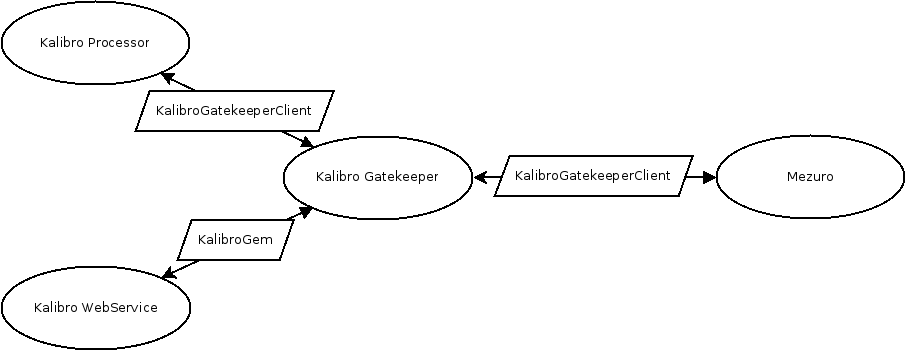
\includegraphics[scale=0.35]{images/mezuro-architecture-actual.png}
      \end{center}
    \end{figure}
  \end{frame}

  \begin{frame}
    \frametitle{Arquitetura}
    \framesubtitle{Visão geral - Planejada}

    \begin{figure}[htb]
      \begin{center}
        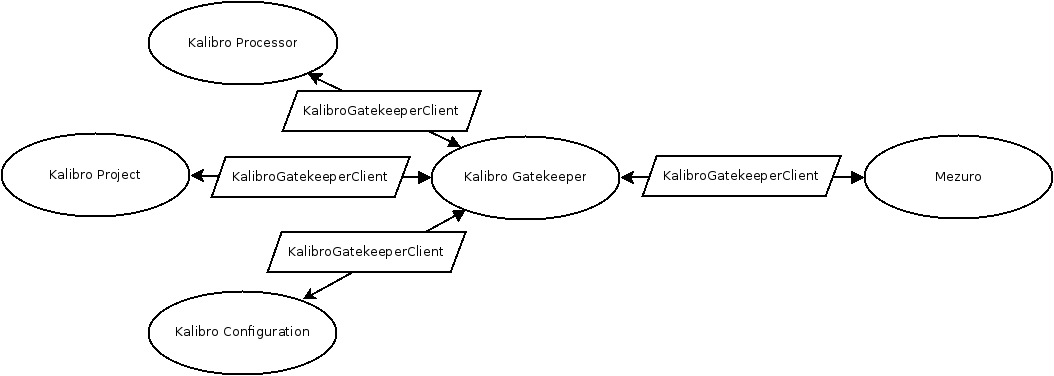
\includegraphics[scale=0.30]{images/mezuro-architecture-predicted.png}
      \end{center}
    \end{figure}
  \end{frame}

  \subsection{Demonstração}
  \begin{frame}
    \frametitle{Criação e processamento de repositório}
    \framesubtitle{Projeto}

    \begin{figure}[htb]
      \begin{center}
        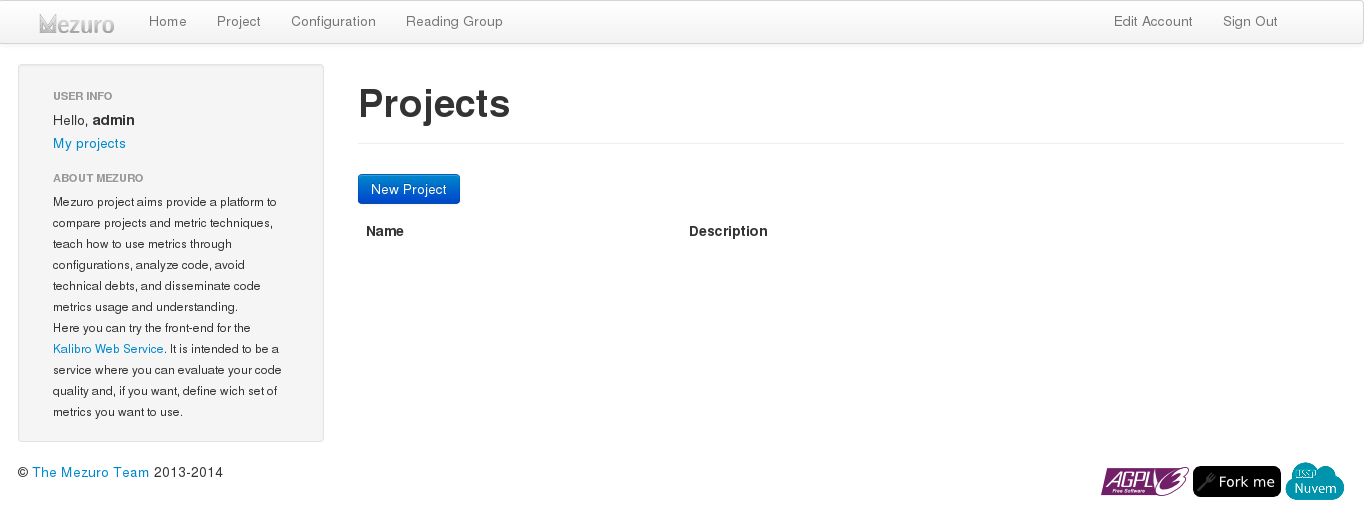
\includegraphics[scale=0.24]{images/00-new-project.png}
      \end{center}
    \end{figure}
  \end{frame}

  \begin{frame}
    \frametitle{Criação e processamento de repositório}
    \framesubtitle{Projeto - Formulário}

    \begin{figure}[htb]
      \begin{center}
        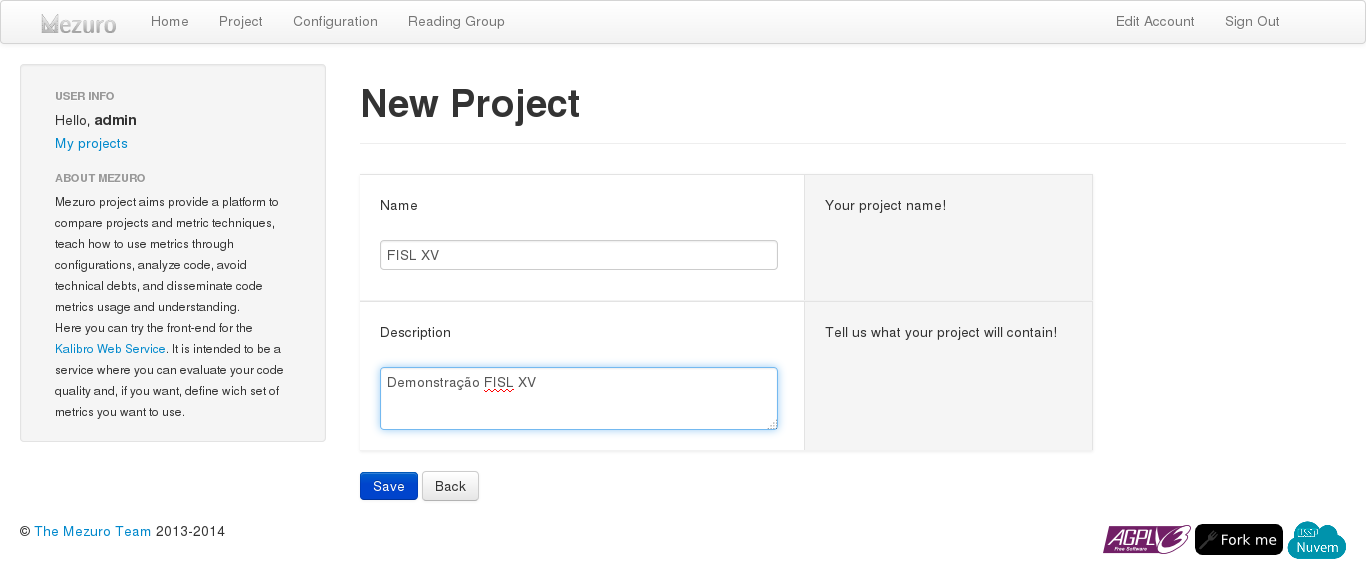
\includegraphics[scale=0.24]{images/01-new-project-form.png}
      \end{center}
    \end{figure}
  \end{frame}

  \begin{frame}
    \frametitle{Criação e processamento de repositório}
    \framesubtitle{Projeto - Criado}

    \begin{figure}[htb]
      \begin{center}
        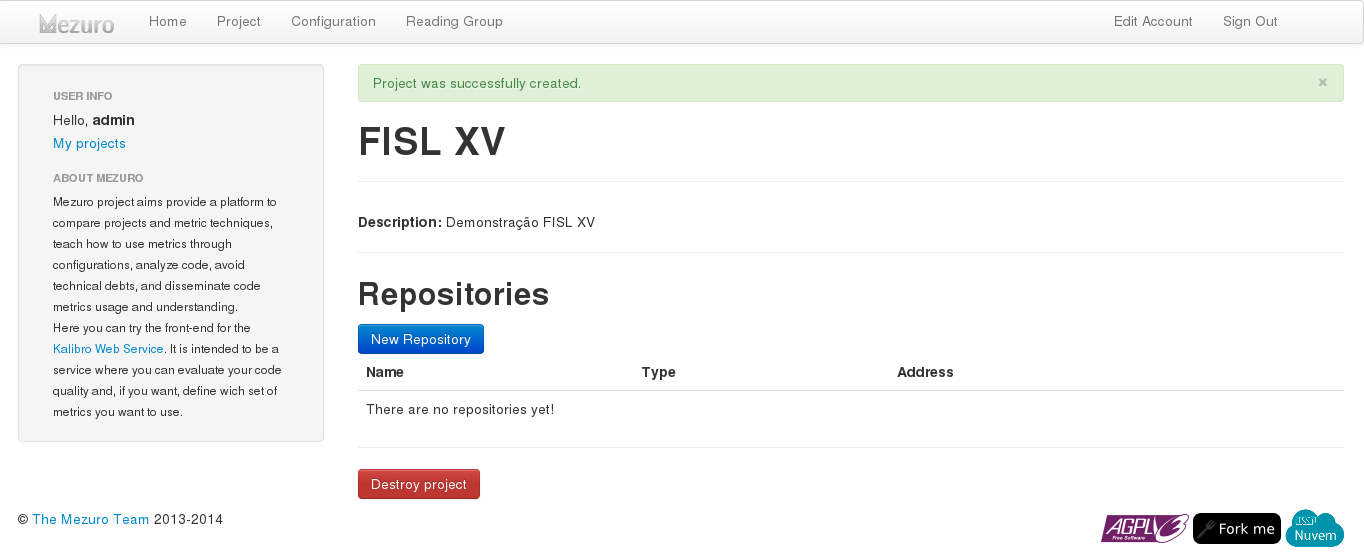
\includegraphics[scale=0.24]{images/02-new-project-created.png}
      \end{center}
    \end{figure}
  \end{frame}

  \begin{frame}
    \frametitle{Criação e processamento de repositório}
    \framesubtitle{Repositório}

    \begin{figure}[htb]
      \begin{center}
        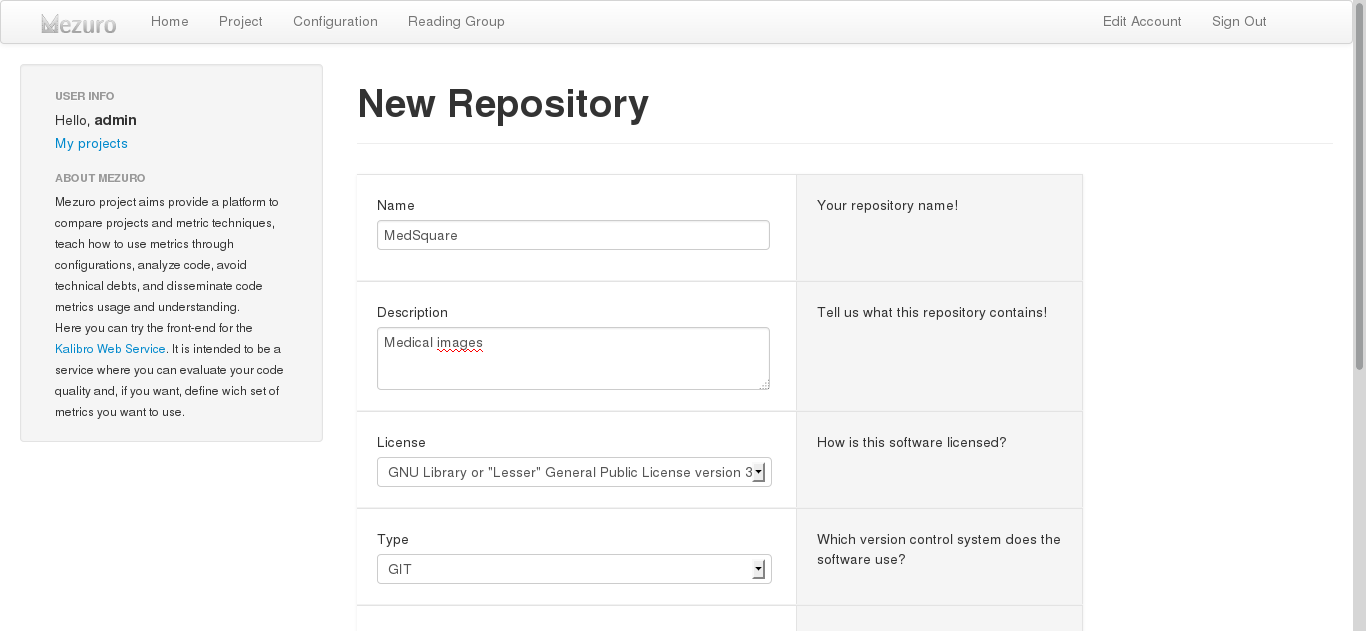
\includegraphics[scale=0.24]{images/03-new-repository-form.png}
      \end{center}
    \end{figure}
  \end{frame}

  \begin{frame}
    \frametitle{Criação e processamento de repositório}
    \framesubtitle{Exibição de resultados}

    \begin{figure}[htb]
      \begin{center}
        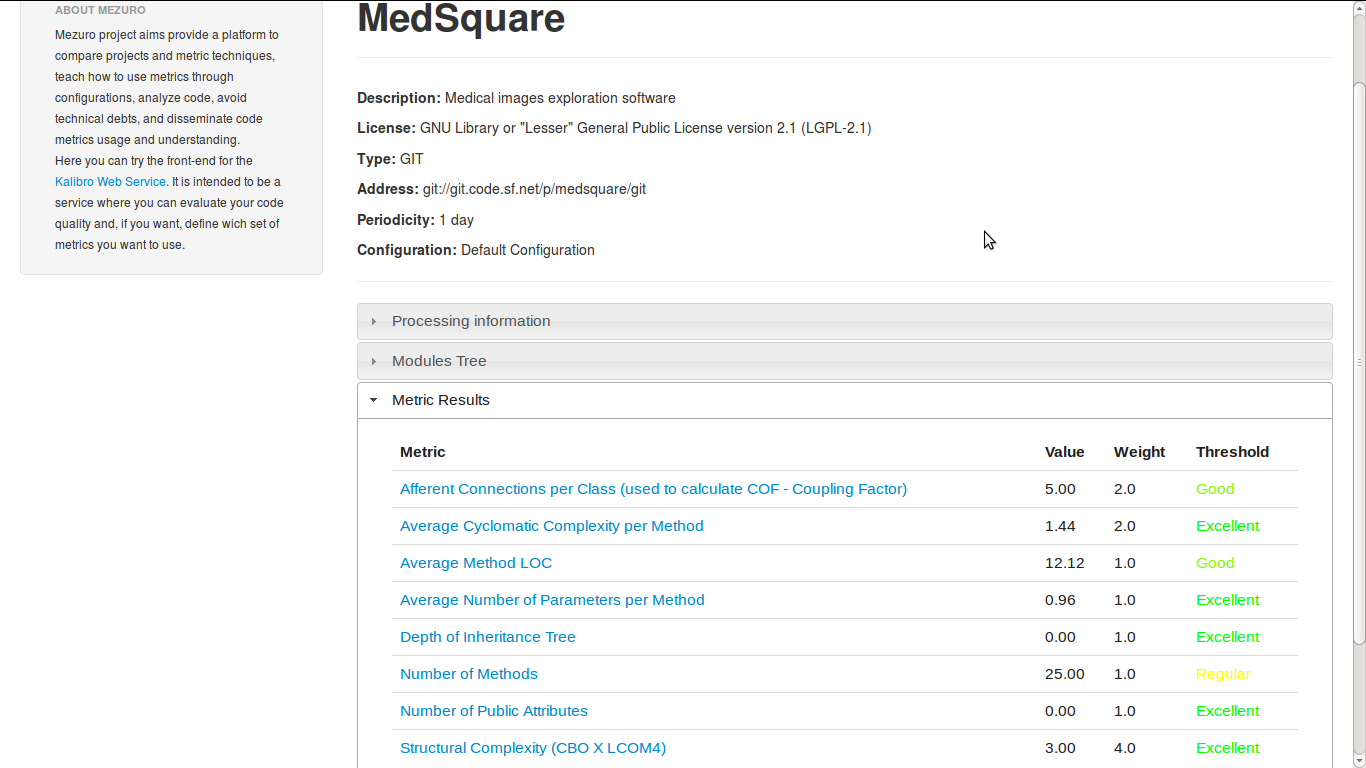
\includegraphics[scale=0.24]{images/04-new-repository-results.png}
      \end{center}
    \end{figure}
  \end{frame}

  \begin{frame}
    \frametitle{Criação de configuração}
    \framesubtitle{Configuração}
  \end{frame}

  \begin{frame}
    \frametitle{Criação e processamento de repositório}
    \framesubtitle{Escolha de métrica e interpretação}
  \end{frame}

\section{Software Público}
\begin{frame}
  \LARGE{\textbf{Software Público}}
\end{frame}

\section{Conclusão}
\begin{frame}
  \frametitle{Conclusão}
  \framesubtitle{}

  \LARGE{\textbf{Conclusão}}
\end{frame}

\begin{frame}
  \frametitle{Conclusão}
  \framesubtitle{Revisão}

  \begin{itemize}
    \item \textbf{Métricas}
      \begin{itemize}
        \item Existem diversas ferramentas que extraem informações sobre a qualidade do código-fonte
        \item Mas ainda não sabemos classificar o que é bom e o que é ruim
        \item Incorporar isto ao processo de desenvolvimento pode aumentar a qualidade
      \end{itemize}
    \item \textbf{Plataformas de coleta e interpretação}
      \begin{itemize}
        \item SonarQube e Code Climate
        \item Têm suas qualidades, mas ainda não exatamente o que queremos
      \end{itemize}
    \item \textbf{Mezuro}
      \begin{itemize}
        \item Livre
        \item Flexível
        \item Extensível
        \item Usabilidade
      \end{itemize}
  \end{itemize}
\end{frame}

\begin{frame}
  \frametitle{Conclusão}
  \framesubtitle{Próximos passos}

  \begin{enumerate}
    \item Terminar o Kalibro Processor
    \item Utilizar em produção
    \item Obter usuários ``reais''
    \item Continuar a refatoração do Kalibro até alcançar a arquitetura planejada
    \item Obter contribuidores independentes
  \end{enumerate}
\end{frame}

\begin{frame}
  \frametitle{Conclusão}
  \framesubtitle{Nos acompanhe}

  \begin{itemize}
    \item \url{http://mezuro.org}
    \item \url{https://www.github.com/mezuro}
  \end{itemize}

  \LARGE{\textbf{Obrigado!}}
\end{frame}
\end{document}